\documentclass{article}

\usepackage[a4paper, margin=20mm]{geometry}
\usepackage{amsmath}
\usepackage{amsthm}
\usepackage{amssymb}
\usepackage{graphicx}
\usepackage{enumitem}

\def\c#1{\texttt{#1}}

\title{Homework 3 - Information Security (ICS344)}
\author{Alfaifi, Ammar -- 201855360}
\date{Nov. 11, 2023}

\begin{document}

\maketitle

\section{Man-In-The-Middle Attack using ARP Cache Poisoning} % (fold)
\label{sec:setup}
For the IP and MAC addresses, see Figure~\ref{fig:A-ip}, Figure~\ref{fig:B-ip}, and Figure~\ref{fig:M-ip}.

\begin{figure}[!hb]
	\centering
	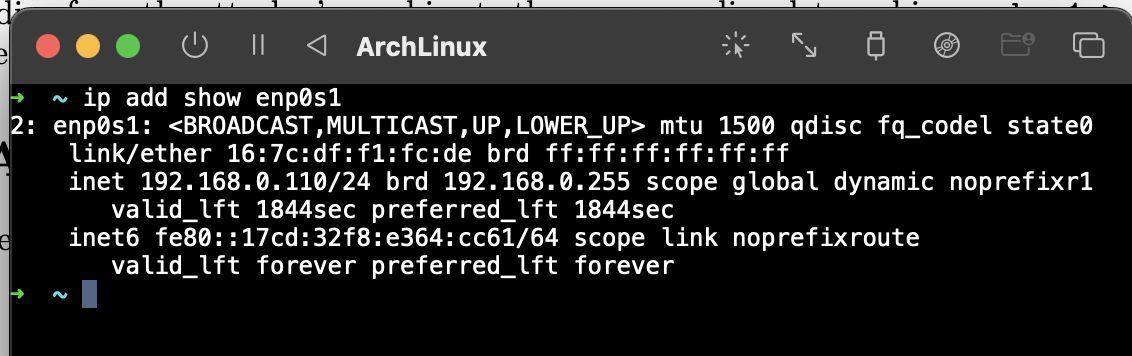
\includegraphics[width=0.8\textwidth]{figures/A-ip.png}
	\caption{IP and MAC addresses for the victim machine \c{A}, }
	\label{fig:A-ip}
\end{figure}

\begin{figure}[!hb]
	\centering
	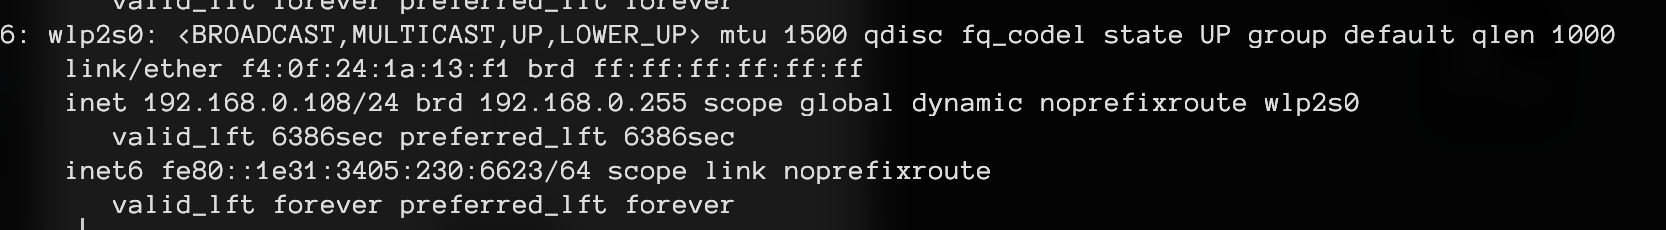
\includegraphics[width=0.8\textwidth]{figures/B-ip.png}
	\caption{IP and MAC addresses for machine \c{B}, }
	\label{fig:B-ip}
\end{figure}

\begin{figure}[!hb]
	\centering
	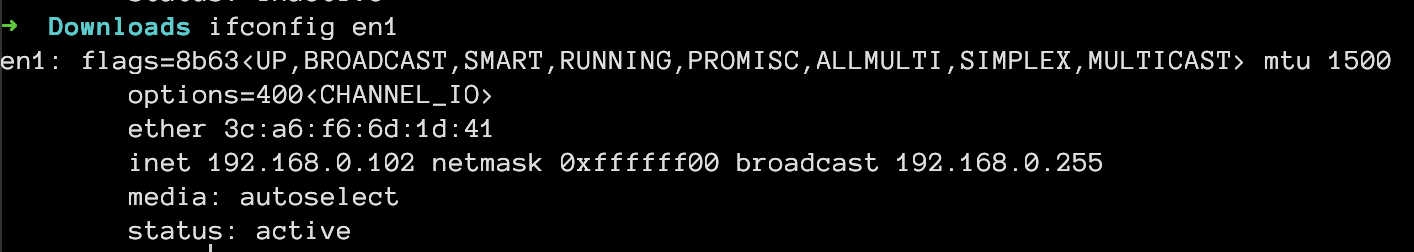
\includegraphics[width=0.8\textwidth]{figures/M-ip.png}
	\caption{IP and MAC addresses for MITM machine \c{M}, }
	\label{fig:M-ip}
\end{figure}

\subsection{ARP Table Poisoning} % (fold)
\label{sub:ARP Table Poisoning}
Before the ARP table poisoning is carried see the victim ARP table in Figure~\ref{fig:A-arp}. Then after the code in Figure~\ref{fig:poisoning-code} is executed to poisin victim's ARP table, we see in Figure~\ref{fig:A-arp-piosined} B's MAC address is now M's one.

\begin{figure}[hb]
	\centering
	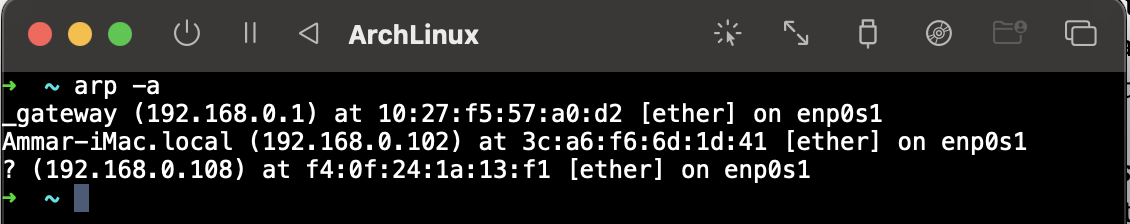
\includegraphics[width=0.8\textwidth]{figures/A-arp.png}
	\caption{This shows the ARP table before poisoning, firt row is the gatway, the second is MITM machin (\c{M}), and the third is the machine \c{B}.}
	\label{fig:A-arp}
\end{figure}
\begin{figure}[hb]
	\centering
	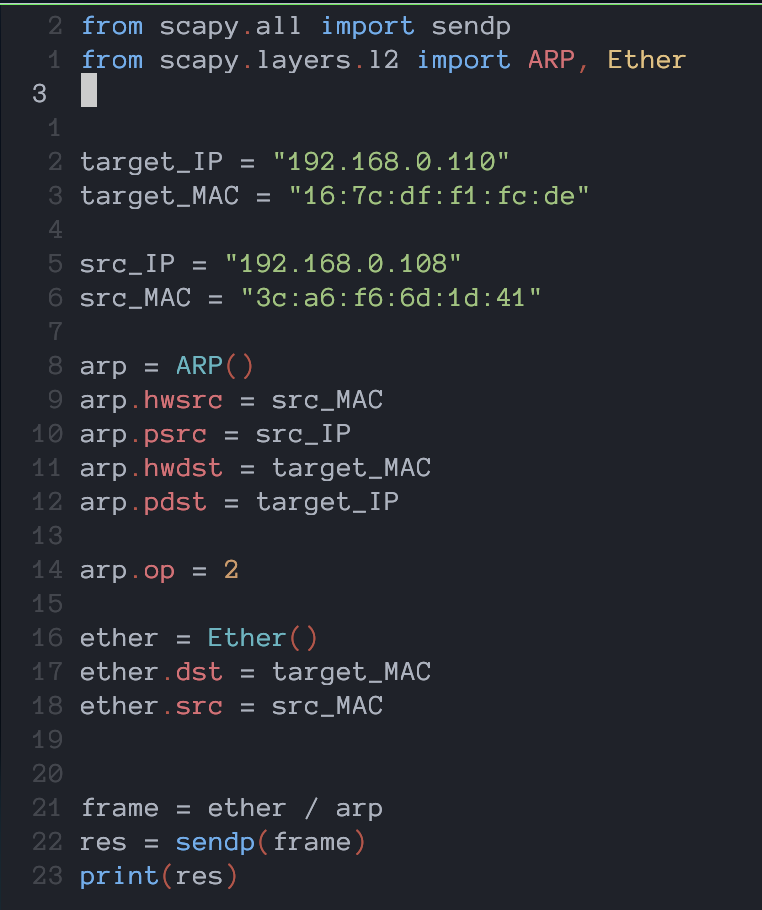
\includegraphics[width=0.4\textwidth]{figures/poisin-code.png}
	\caption{\c{scapy} code I use to poisin machine's A ARP table. It sends a response ARP message (\c{op=2}) as if it comes from machine B, telling victim B' MAC address. However it's M's MAC address. Hence, forwarding traffic from \c{A} to \c{M}, instead of from \c{A} to \c{B}, normally.}
	\label{fig:poisoning-code}
\end{figure}
\begin{figure}[hb]
	\centering
	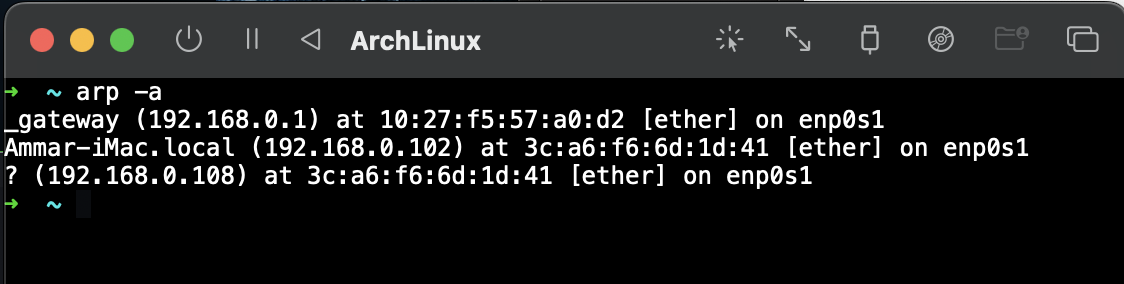
\includegraphics[width=0.7\textwidth]{figures/A-arp-piosined.png}
	\caption{A's ARP table after poisoning. See A's MAC address (3rd row) is that of M (the attacker).}
	\label{fig:A-arp-piosined}
\end{figure}
% subsection ARP Table Poisoning (end)

\newpage
\subsection{Build UDP Packet} % (fold)
\label{sub:Build UDP Packet}
The following code nippet will construct a UDP packet sent from machine \c{A} to machine \c{B}, refer to
Section~\ref{sec:setup} for information about the IP addresses used.
\begin{verbatim}
from scapy.all import *
packet = (
    IP(src="192.168.0.110", dst="192.168.1.108")
    / UDP(sport=1234, dport=5678)
    / "Ammar Alfaifi"
)
send(packet)
\end{verbatim}
See Figure~\ref{fig:udp-output} for the output of this code.
\begin{figure}[hb]
	\centering
	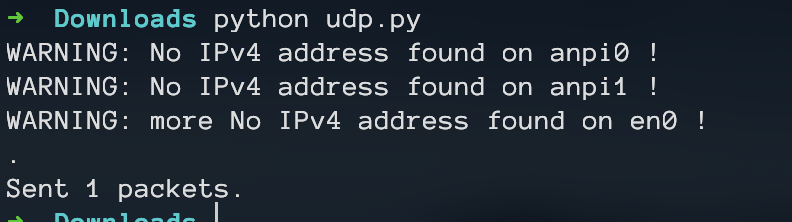
\includegraphics[width=0.7\textwidth]{figures/udp-output.png}
	\caption{Output after executing \c{scapy} code to construct and send a UDP packet from \c{A} to \c{B}}
	\label{fig:udp-output}
\end{figure}
% subsection Build UDP Packet (end)


\subsection{Sniffing and Spoofing UDP} % (fold)
\label{sub:Sniffing and Spoofing UDP}
As in Figure~\ref{fig:spoofed} we recive UDP message containing my name, then I reversed it and sent it thru network. The code used is shown in Figure~\ref{fig:spoof-code}.
\begin{figure}[hb]
	\centering
	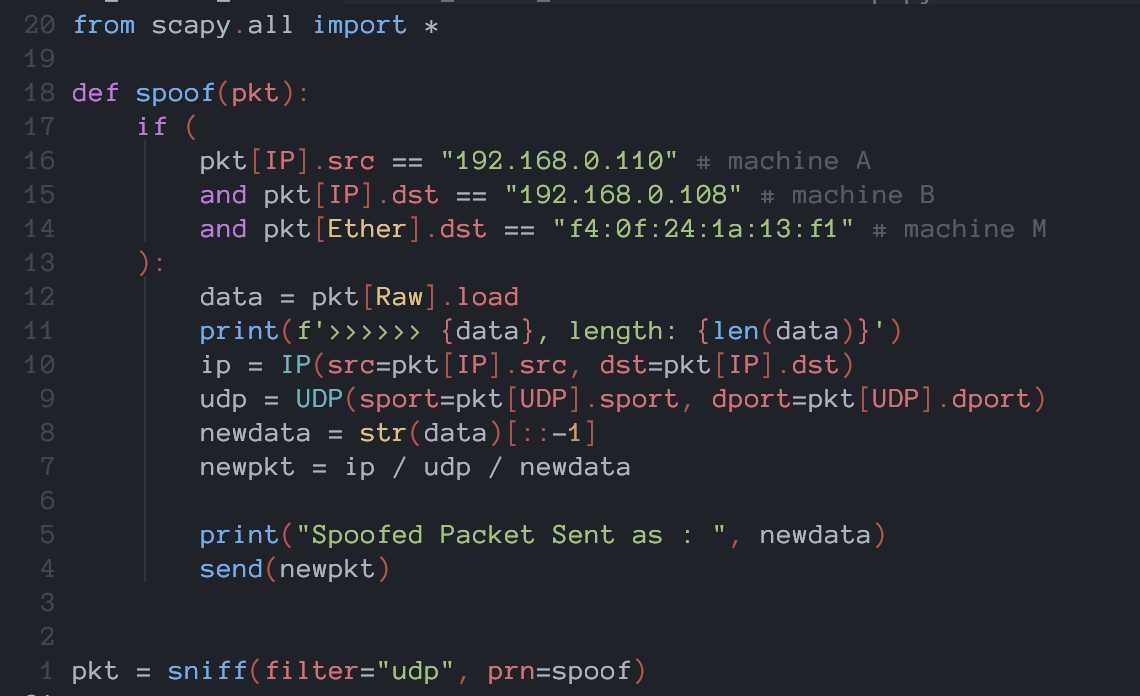
\includegraphics[width=0.7\textwidth]{figures/spoof-code}
	\caption{Shows the scapy code to sniff and then spoof a UDP packet.}
	\label{fig:spoof-code}
\end{figure}

\begin{figure}[hb]
	\centering
	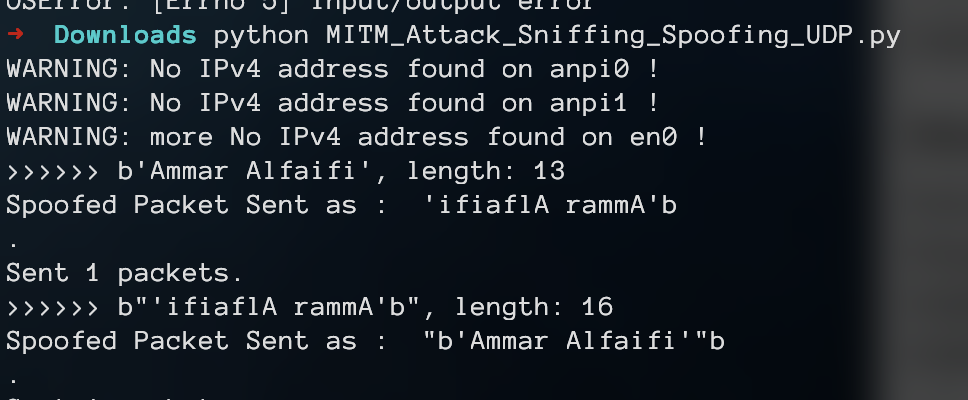
\includegraphics[width=0.8\textwidth]{figures/spoof.png}
	\caption{Spoof code output it shows the original message as well as the the spoofed one.}
	\label{fig:spoofed}
\end{figure}

% subsection Sniffing and Spoofing UDP (end)
% section Man-In-The-Middle Attack using ARP Cache Poisoning (end)

\newpage
\section{Man-In-The-Middle Attack with Ciphertext} % (fold)
\label{sec:Man-In-The-Middle Attack with Ciphertext}
As in Section~\ref{sec:setup}, we poisoned A's ARP table to redirect UDP packets, going to B, to M.

\subsection{Encrypt UDP Body} % (fold)
\label{sub:Encrypt UDP Body}
Figure~\ref{fig:send-udp-enc} shows the \c{scapy} code to send an encrypted message within UDP packet
from machine A to machine B. Also, see Figure~\ref{fig:scapy-run} for this code output.

\begin{figure}[!hb]
	\centering
	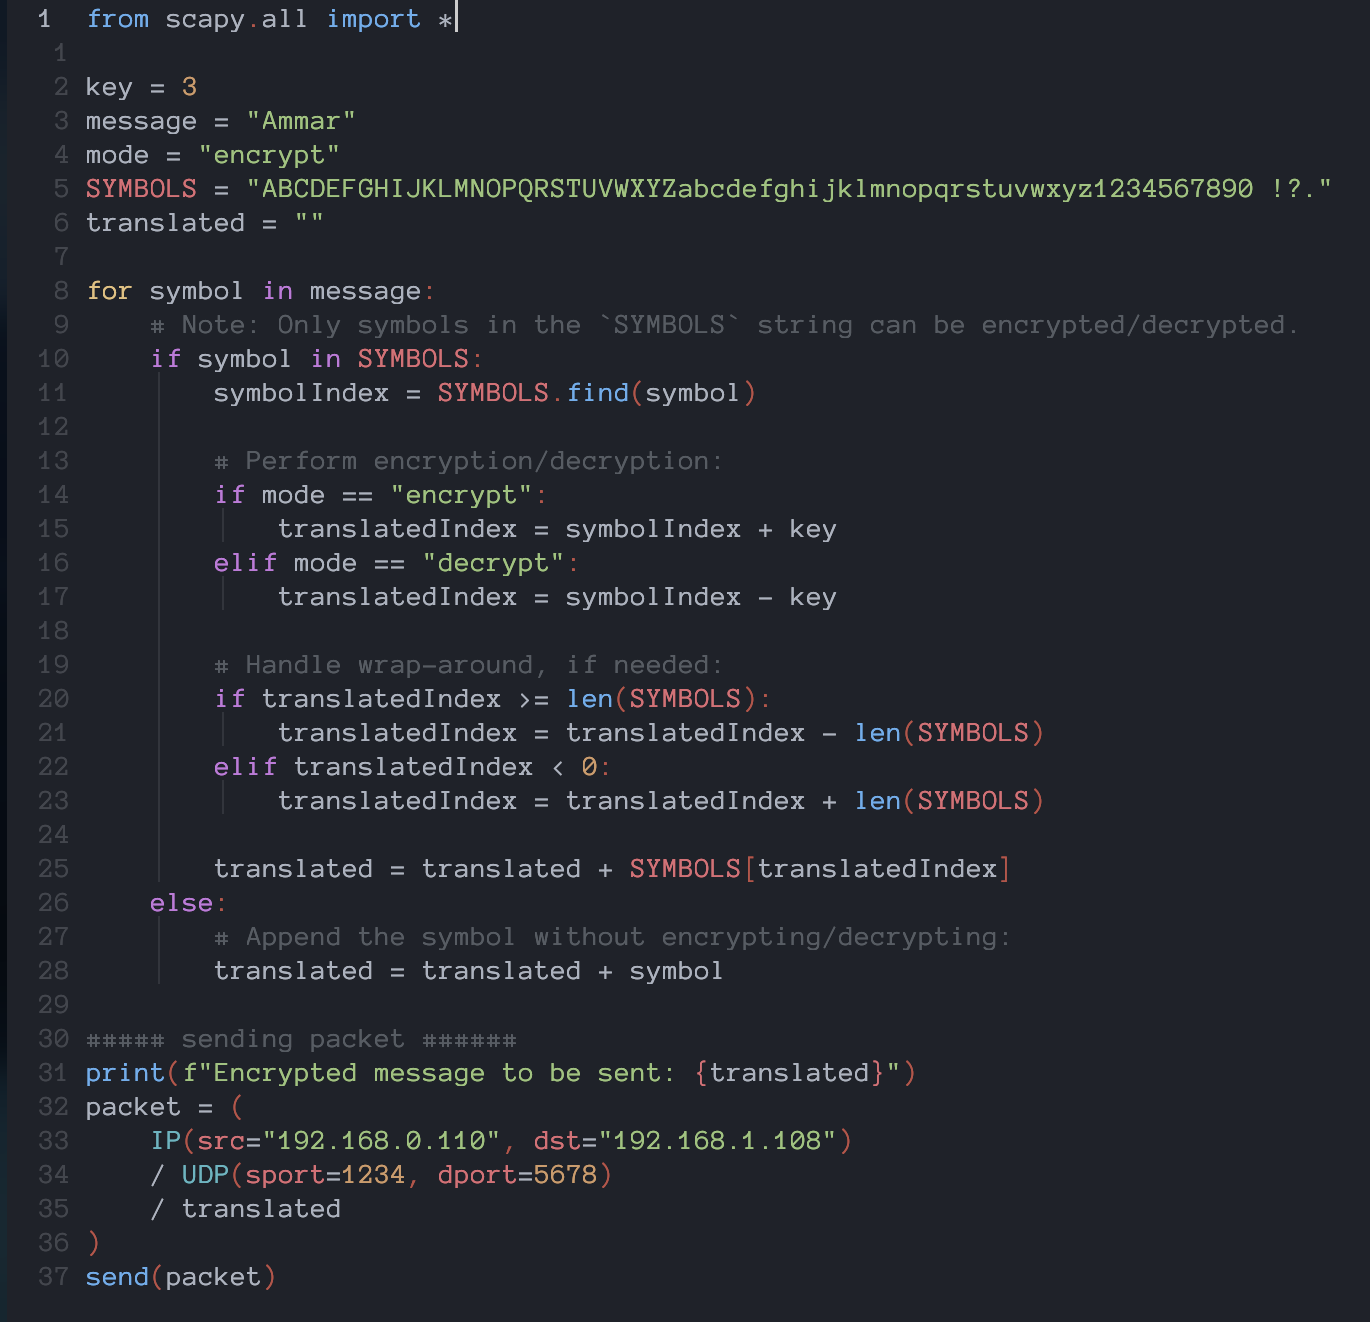
\includegraphics[width=0.8\textwidth]{figures/udp-enc}
	\caption{Code to send a UDP packet but the message (i.e., "Ammar") is now encrypted.}
	\label{fig:send-udp-enc}
\end{figure}

\begin{figure}[!hb]
	\centering
	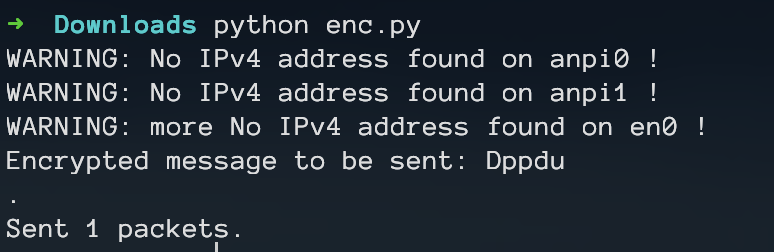
\includegraphics[width=0.5\textwidth]{figures/send-udp-enc}
	\caption{Result of running scapy code}
	\label{fig:scapy-run}
\end{figure}
% subsection Encrypt UDP Body (end)

\subsection{Encrypted UDP in Wireshark} % (fold)
\label{sub:Encrypted UDP in Wireshark}
See Figure~\ref{fig:enc-udp-wire} for wire for our encrypted UDP packet,
showing tha same body as in the scapy outp, Figure~\ref{fig:udp-output}.
\begin{figure}[!hb]
	\centering
	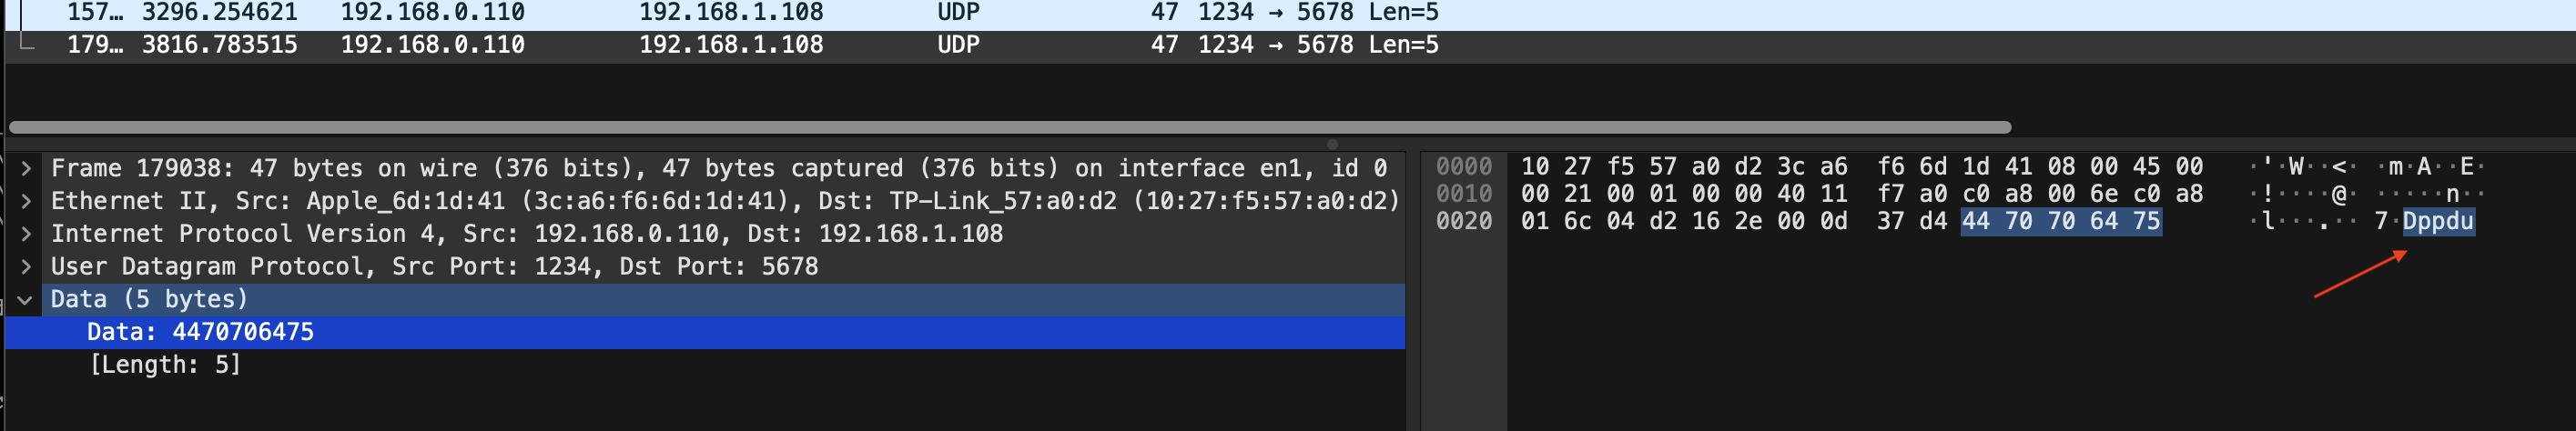
\includegraphics[width=0.8\textwidth]{figures/enc-udp-wire}
	\caption{We see the packet details, with its encrypted message.}
	\label{fig:enc-udp-wire}
\end{figure}
% subsection Encrypted UDP in Wireshark (end)

\subsection{Hacking Encrypted UDP} % (fold)
\label{sub:Hacking Encrypted UDP}
In this step I combine Section~\ref{sec:setup} and Section~\ref{sub:Encrypt UDP Body}, to sniff
a UDP packet and then tries to decrypt the ciphertext. Thse code is shown in Figure~\ref{fig:dec-code} and
the result of the sniffing and decryption is shown in Figure~\ref{fig:dec-res}.

\begin{figure}[!hb]
	\centering
	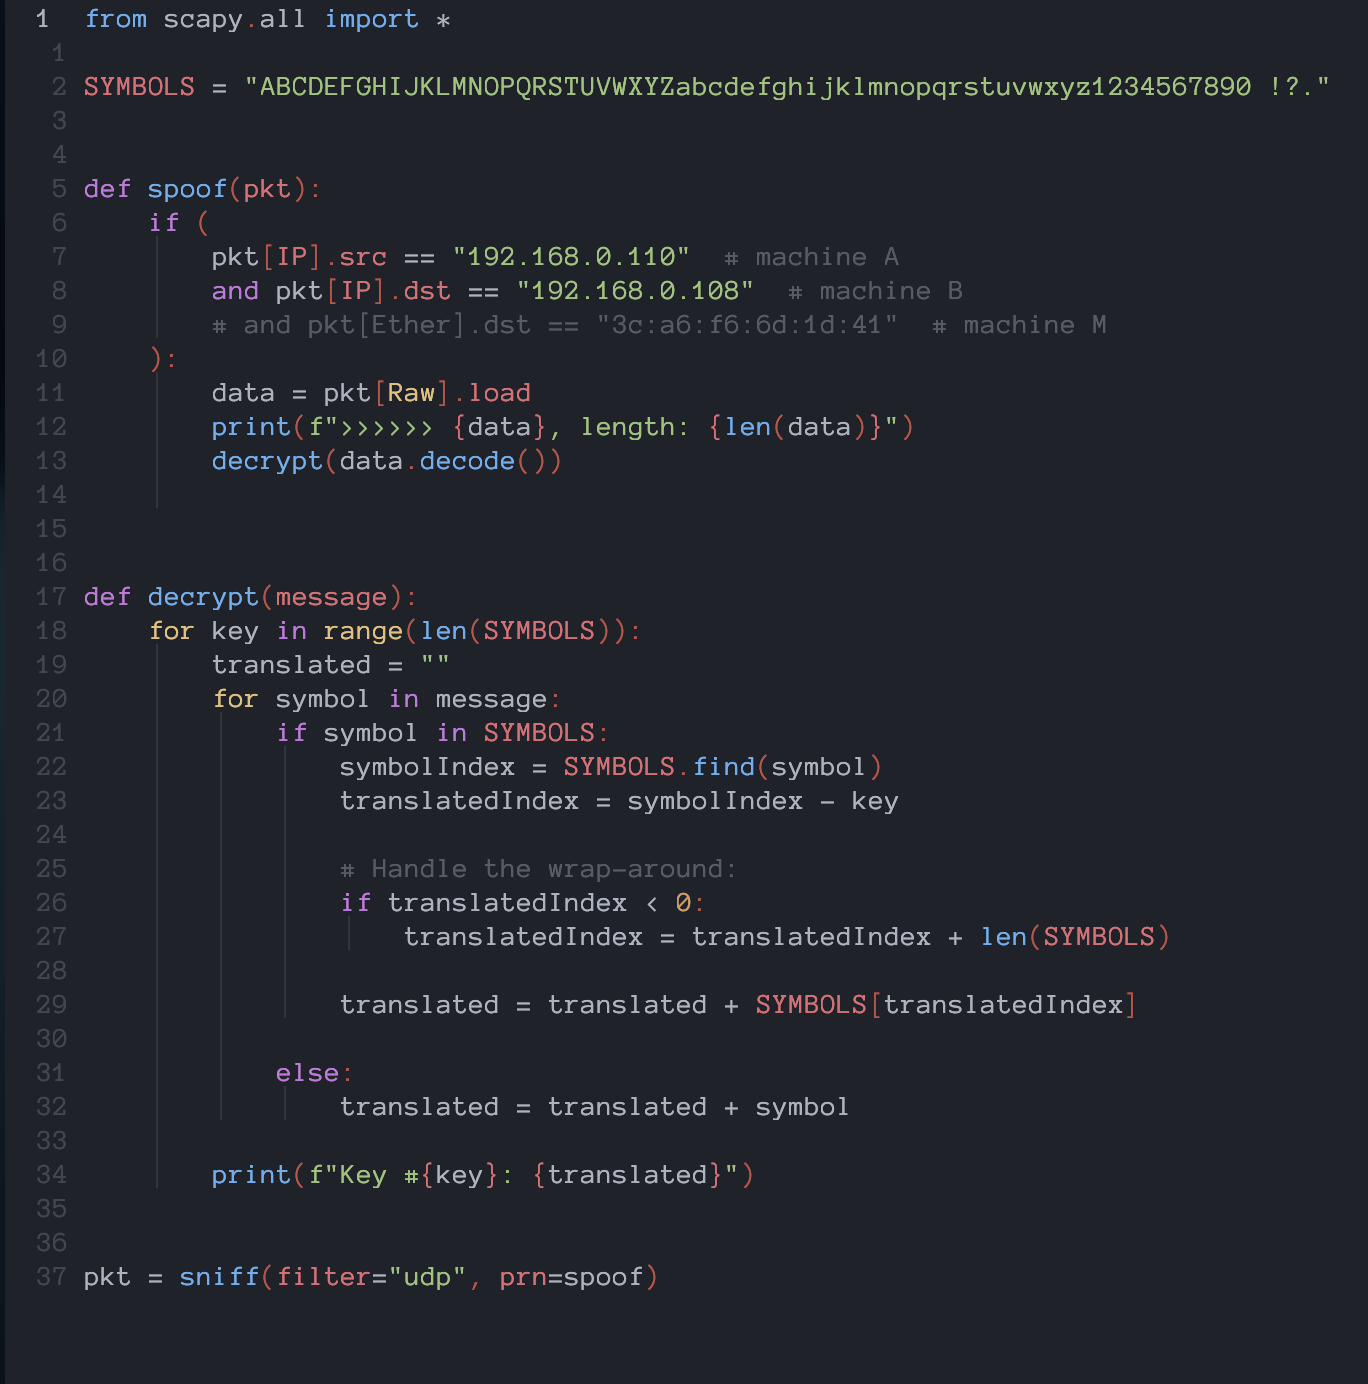
\includegraphics[width=0.6\textwidth]{figures/dec-code}
	\caption{It shows hacking code that sniffs first then try to decrypt the message.}
	\label{fig:dec-code}
\end{figure}

\begin{figure}[!hb]
	\centering
	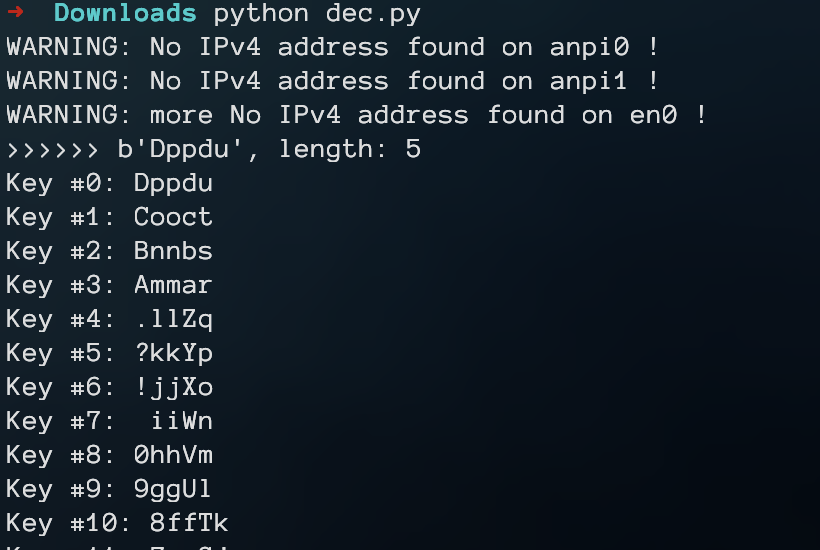
\includegraphics[width=0.6\textwidth]{figures/dec-res}
	\caption{The result of trying to find the correct additive key, we see that my name is recovered with 
  key equals 3, as the original encrypting key.}
	\label{fig:dec-res}
\end{figure}
% subsection Hacking Encrypted UDP (end)
% section Man-In-The-Middle Attack with Ciphertext (end)

\section{Modern Cipher and Message Digest} % (fold)
\label{sec:Modern Cipher and Message Digest}
\subsection{Encoding}

Encoding is a process of converting data into a different format using a scheme that is publicly available. It is not meant for security purposes but rather for data integrity and efficiency. Common encoding schemes include Base64 and URL encoding.

\paragraph{Example}

Let's encode the string "Hello, World!" using Base64.

\texttt{Hello, World! $\rightarrow$ SGVsbG8sIFdvcmxkIQ==}

\subsection{Encryption}

Encryption involves transforming data into a secure format using a key, making it unreadable without the corresponding decryption key. It is designed for confidentiality and privacy. Common encryption algorithms include AES and RSA.

\paragraph{Example}

Encrypt the message "Confidential Data" using the \c{aes-128-cbc} and "1234" as the secret algorithm with a key.

\texttt{Original: Confidential Data}

\texttt{Encrypted: cxrv5ZR2lGIq/PQTPvDlCieQ9QDDg7VbTvGlLja8clw=}

\subsection{Hashing}

Hashing is a one-way process that generates a fixed-size string of characters (hash) from input data. It is used for data integrity and quick data retrieval but is not reversible. Common hashing algorithms include SHA-256 and MD5.

\paragraph{Example}

Hash the password "SecurePassword" using the SHA-256 algorithm.

\texttt{SecurePassword $\rightarrow$ c89bbbf01fa7840fdbf194a621ef899258e9210d6c77b6f033b6ebfa15f7230d}
% section Modern Cipher and Message Digest (end)



\end{document}
